\documentclass[11pt]{article}


\newcommand{\putdraft}{\special {!userdict begin /bop-hook{gsave 200 30
translate 65 rotate /Times-Roman findfont 216 scalefont setfont 0 0
moveto 0.9 setgray (DRAFT) show grestore}def end}}

\def\quote{\list{}{\rightmargin\leftmargin}\item[]}
\let\endquote=\endlist

\def\changemargin#1#2{\list{}{\rightmargin#2\leftmargin#1}\item[]}
\let\endchangemargin=\endlist

%%% use the geometry package to specify the margins.  up the
%%% headheight a bit to give more room for the headers
\usepackage{hyperref}
\usepackage[head=12pt]{geometry}
\usepackage{graphicx}
\usepackage{amsmath}
\usepackage{upgreek}

%%% the possible options to the memo package are:
%%%
%%%  NofM - output pagenumbers as N / M, where M is the last page.
%%%         This requires two LaTeX runs.  Only works if fancy is specified
%%%
%%%  prerule - draw a rule between the memo preamble and the memo body
%%%
%%%  fancy - use the fancyhdr package to make nice page headers and footers
%%%          if you don't like the default, go ahead and override the
%%%          fancyhdr stuff directly.  The default handles twosided
%%%          documents.
%%%
%%%  rcs - use the rcsinfo package to generate the contents of the Date,
%%%        Version, and File memo header fields.  This is very useful
%%%        if you are using the RCS package to manage your text.
%%%        You will have to put the following text in your file:
%%%
%%%             \rcsInfo $Id$
%%%
%%%        It will be updated by RCS when you commit your changes.
%%%        If you don't specify rcs, the above line will cause LaTeX
%%%        to complain. You will get all three fields with this option.
%%%        You can override the contents of the fields by specifying
%%%        them explicitly. To delete them, use \DeleteMemoField, e.g.:
%%%
%%%             \DeleteMemoField{File}
%%%
\def\tablenotemark#1{\rlap{$^{\rm #1}$}}
%%% This template shows off all of the options
%%% If you're not using RCS, remove the rcs option.
\usepackage[prerule]{memox}

%%% grab the CXC letterhead, specifying the CfA address
\usepackage[addr=cfa]{cxc_letterhead}
%%% and tell the memo package to use it
\memoletterhead{\CXCletterhead}

\begin{document}

\newcommand{\chandra}{{\em Chandra}}
\newcommand{\rosat}{{\em ROSAT}}
\newcommand{\chase}{{\em ChASeM33}}
\newcommand{\etal}{{\em et al.}}
\newcommand{\be}{\begin{enumerate}}
\newcommand{\ee}{\end{enumerate}}
\newcommand{\bc}{\begin{center}}
\newcommand{\ec}{\end{center}}
\newcommand{\bi}{\begin{itemize}}
\newcommand{\ei}{\end{itemize}}
\newcommand{\bd}{\begin{description}}
\newcommand{\ed}{\end{description}}
\newcommand{\bt}{\begin{tabbing}}
\newcommand{\et}{\end{tabbing}}
\newcommand{\code}[1]{\texttt{#1}}

%%% First, define the fields in the memo preamble (i.e, To, From, etc.).
%%% present is \From.
%%%
%%%  \Date - there are two possible places for the date to be printed;
%%%         if this macro is used, a Date: field is output.  If not,
%%%         the string passed to the \memo macro is placed above the
%%%         memo preamble.
%%%
%%%  \From - the author of the memo.
%%%
%%%  \To   - the recipient(s)
%%%
%%%  \Subject - the memo subject (the Subject field)
%%%
%%%  \RE - the Re field
%%%
%%%  \ShortSubj - a short subject to be output in the page header, if the
%%%               fancy package option was specified.  If this isn't specified,
%%%               either the Subject or the Re field data will be used.
%%%
%%%  \Cc - a carbon copy list
%%%
%%%  \File - the name of the file which generated this memo. This is output
%%%          in a smaller (typewriter) font
%%%
%%%  \Version - the version of this memo.  This is output in a smaller font
%%%
%%% The macros place their arguments in other macros with the same name,
%%% but prefixed with the word `memo' (e.g., \memoFrom).  You can use
%%% these if you choose to redefine the page headers and footers.
%%%
%%% If for some reason you've defined a field and you wish to delete
%%% it, use the \DeleteMemoField macro.
%%%
%%%             \DeleteMemoField{File}
%%%
%%% It is harmless to delete a field which hasn't had a value assigned
%%% to it. Assigning an empty value to a field will not delete it.
%%%
%%% You can define a field as many times as you'd like.


%%% remove this line if you're NOT using the rcs option, otherwise
%%% you'll get errors
%\putdraft
\Subject{Estimation of Potential Polymerization of ACIS OBF Contaminant}
%\RE{The message you last sent me}
%\ShortSubj{ }
\From{John A. ZuHone}
\To{Chandra Operations Team}
%\Cc{ }

%%% This template uses the RCS information for the Date, Version, and
%%% File fields.  You can override them individually by explicitly
%%% defining them.

%\File{ }

%\Version{1.0}
\Date{\today}

%%% Generate the memo header.  If the \Date macro isn't specified,

\memo{}

\section{Abstract}

A contamination layer has built up on the ACIS Optical Blocking Filters over the
lifetime of the \chandra~mission. A bakeout of the ACIS instrument could potentially
drive the contaminant off the filters, but this will be extremely difficult if the
contaminant has been significantly polymerized by exposure to ultraviolet light.
This memo is presented to support the conclusion that the filters have been exposed
to insufficient ultraviolet light over the duration of the mission to significantly
polymerize the contaminant.

%%% If you wish to redefine the page headers and footers, do so here.
\section{Introduction}
%%% The body of the memo.  No text should appear above here.

It was noticed early in the mission that the low-energy sensitivity of ACIS is
decreasing with time. It has been determined that the loss of effective area is
due to a contamination layer building up on the surface of the Optical Blocking
Filters (OBFs) facing the spacecraft interior. The contamination layer continues
to accumulate even after 16 years on orbit. The accumulation rate, the chemical
composition, and the spatial distribution of the contaminant have all varied with
time over the mission.

In 2004, the CXO project considered a ``bakeout'' of the ACIS instrument to remove
the contaminant, but it was decided it was not worth the risk, and shortly thereafter
the accumulation rate of the contaminant decreased. However, since 2012, the rate of
accumulation of the contaminant has been increasing, raising again the need to consider
a possible bakeout. Figure \ref{fig:contam_buildup} shows the increase in surface mass
density of the contaminant as a function of time over the life of the mission so far.

One factor which would determine the likelihood of a successful bakeout is the volatility
of the contaminant, which is unknown since we do not know its molecular structure. If the
volatility of the contaminant is low, it will be much more difficult to bake it off. One
extreme possibility for a low volatility is if the contaminant is significantly polymerized.
After the first Hubble Space Telescope (HST) servicing mission in 1999, a layer of polymerized
contaminant was discovered on the pick-off mirror. It was subsequently determined that
the polymerization of the material occurred due to ultraviolet (UV) photons breaking molecular
bonds. The primary source of these UV photons was from the Sun, reflected from the bright Earth.

This implies that the contaminant that has built up on the OBFs may have been similarly
polymerized by UV photons. In this memo, we perform an analysis of the various likely
sources of UV flux which have impinged on the OBFs over the lifetime of the mission,
to determine there has been a fluence of UV photons with sufficient energy to polymerize
a significant amount of the contaminant, which could significantly degrade the efficiency
of a potential bakeout of the ACIS OBFs.

\section{Estimation of the Effects of UV Flux}

In this section, we will present a series of calculations of the estimated UV fluence
``observed'' by ACIS from various sources. Our goal is to calculate a ``worst-case'' UV
fluence, which will necessitate a number of simplifying assumptions that will be detailed
throughout this memo.

\begin{figure}
\begin{center}
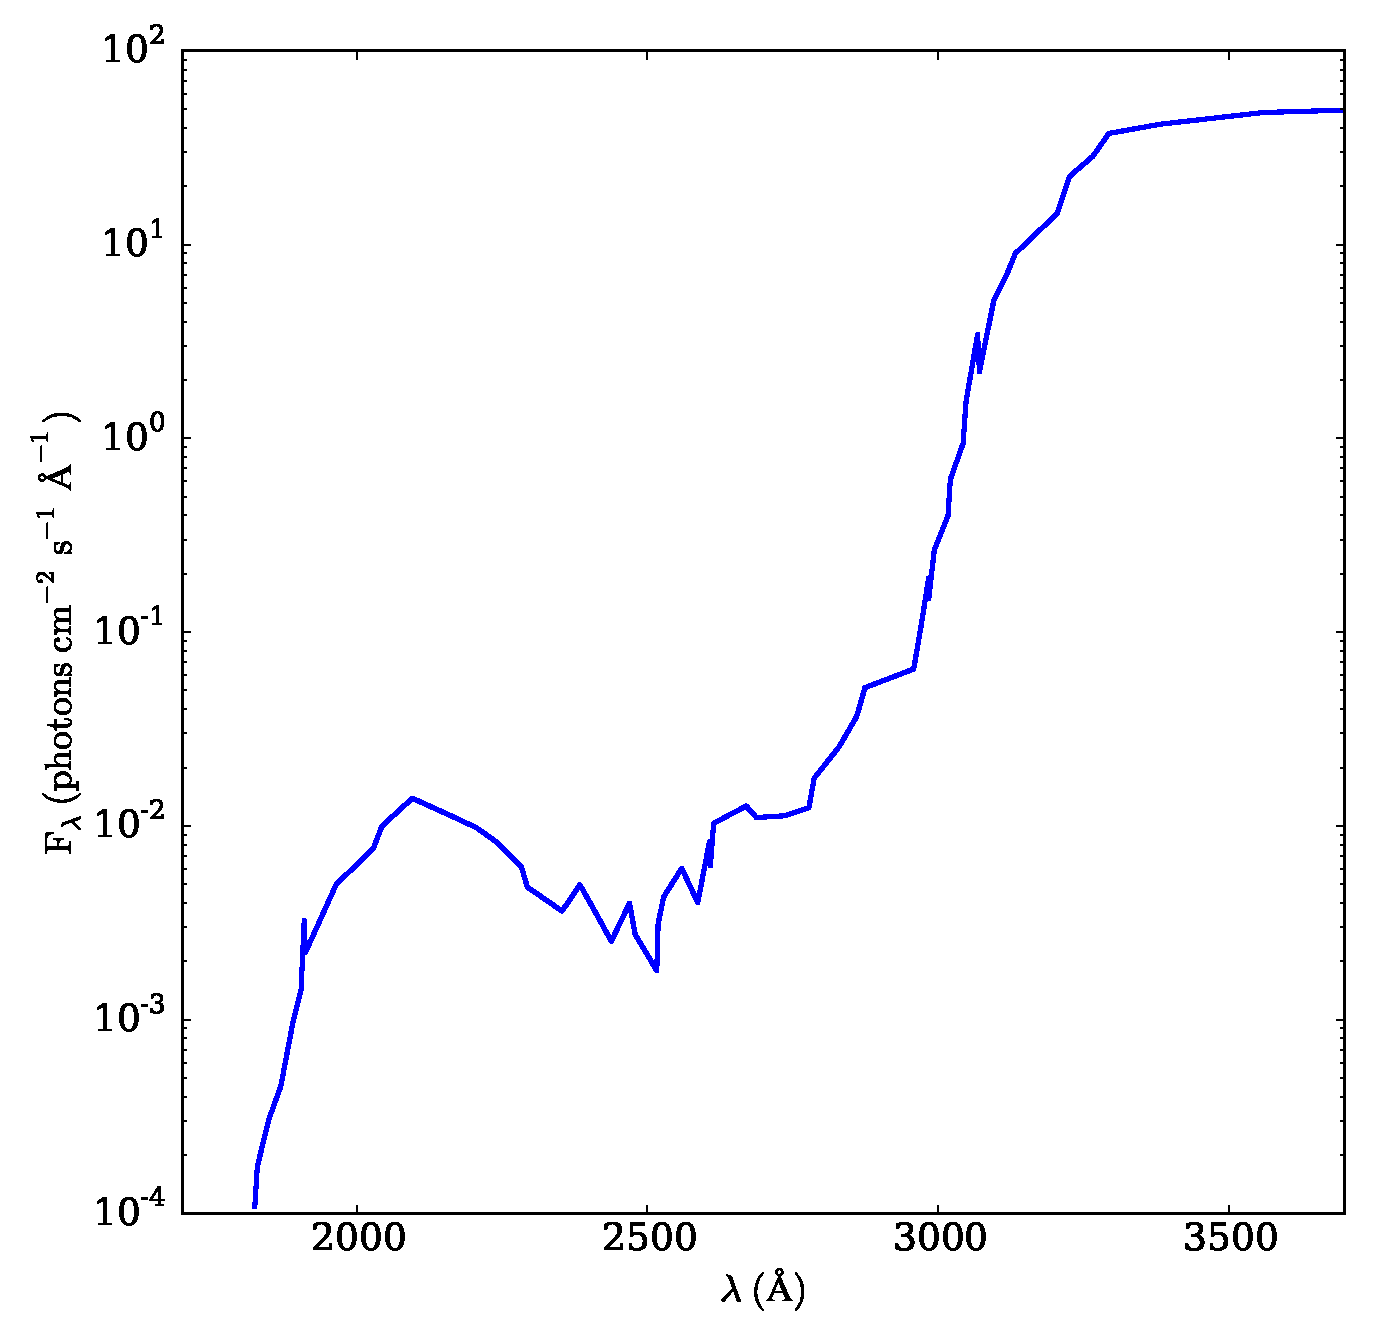
\includegraphics[width=0.7\textwidth]{bright_earth_intensity.eps}
\caption{Specific intensity of solar UV photons backscattered from the bright earth. Dashed
vertical lines show the wavelengths of photon energies that can break H-C and C-C bonds.
Figure reproduced from the HST memo.\label{fig:bright_earth_intensity}}
\end{center}
\end{figure}

\subsection{Assumptions About the Nature of the Contaminant}

Since we do not know the molecular composition of the contaminant, it will be necessary to make
some assumptions. It is known that the contaminant is composed primarily of H and C atoms,
with some amounts of O and F. We will assume that the contaminant is a saturated hydrocarbon,
primarily composed of covalently bonded H and C atoms, with $N_{\rm C}$ C atoms per molecule.

This indicates that H-C or C-C bonds must be broken in order to polymerize the contaminant. The
energies required to break these bonds are $E_{\rm H-C}$ = 99~kcal/mol and $E_{\rm C-C}$ =
83~kcal/mol.\footnote{\url{http://www.cem.msu.edu/~reusch/OrgPage/bndenrgy.htm}} These energies
correspond to photon wavelengths of $\lambda_{\rm H-C}$ = 2888~${\rm \AA}$ and $\lambda_{\rm C-C}$
= 3445~${\rm \AA}$.

\subsection{UV Flux from the Bright Earth}

Our first source of UV flux that we consider is that which is from the Sun, backscattered
from the Earth's atmosphere. Figure \ref{fig:bright_earth_intensity} shows the specific
intensity of these UV photons in the $\sim$1800-3800~${\rm \AA}$ wavelength range. There
are steep drops in intensity around 1900~${\rm \AA}$ and 3000~${\rm \AA}$. By integrating
over wavelength, we determine that the intensity of photons which can break the H-C and C-C
bonds are $I_{\rm H-C}$ = 9.23~photons~s$^{-1}$~cm$^{-2}$~arcsec$^{-2}$ and $I_{\rm C-C}$ =
7132.04~photons~s$^{-1}$~cm$^{-2}$~arcsec$^{-2}$.

Though \chandra~does not directly observe the bright Earth, the Earth can be scanned during
maneuvers. Therefore, in order to determine the total UV fluence reflected from the bright
arth which impinged upon the OBFs, it is necessary to determine the total time accumulated over
the lifetime of the mission when the following two conditions are simultaneously satisfied:

\begin{enumerate}
\item The Earth is in the HRMA field of view
\item ACIS is in the focal plane
\end{enumerate}

We assume that condition 1 is satisfied when the angular radius of the Earth is less than the
angular distance between the Earth and the aimpoint. This was determined by querying
the \code{Ska} engineering archive for the MSIDs \code{Dist\_SatEarth} and \code{Point\_EarthCentAng},
corresponding to the distance between the Earth's center and \chandra~($D_E$) and the angle $\phi_E$ between
the Earth and the aimpoint, respectively. The angular radius of the Earth $\theta_E$ is determined
via $\theta_E = \tan^{-1} (R_\oplus/D_E)$. We assume that condition 2 is satisfied when the TSC
position is $\geq$ -25,000. This can be determined using the MSID \code{3TSCPOS} from the \code{Ska}
archive.

The time resolution of the first two MSIDs in the archive is $\Delta{t} = 5$~min, whereas the resolution
of \code{3TSCPOS} is 32.8~seconds, so the time resolution of the calculation is limited to 5-minute intervals.
This likely results in a modest overestimate of the total length of time that the OBFs have been exposed to
the bright Earth, since the Earth will be entering and exiting the field of view during some of these intervals,
and will not be within it during the entire 5 minutes. We do not seek to quantify this overestimate further, since we are adopting a ``worst-case'' approach to this problem. The total time $\Delta{T}$ during which the ACIS OBFs are exposed to the bright Earth is then calculated by simply summing the time intervals which jointly satisfy these conditions:

\begin{eqnarray}
\Delta{T} &=& \displaystyle\sum_i~\Delta{t_i},~{\rm where}~(\phi_{E,i} \leq \theta_{E,i})~{\rm and}~(\code{3TSCPOS}_i > -25000) \\
\nonumber &=& 2.73~{\rm hr}
\end{eqnarray}

\noindent
Figure \ref{fig:time_accum} shows the accumulation of this time over the duration of the mission.

\begin{figure}
\begin{center}
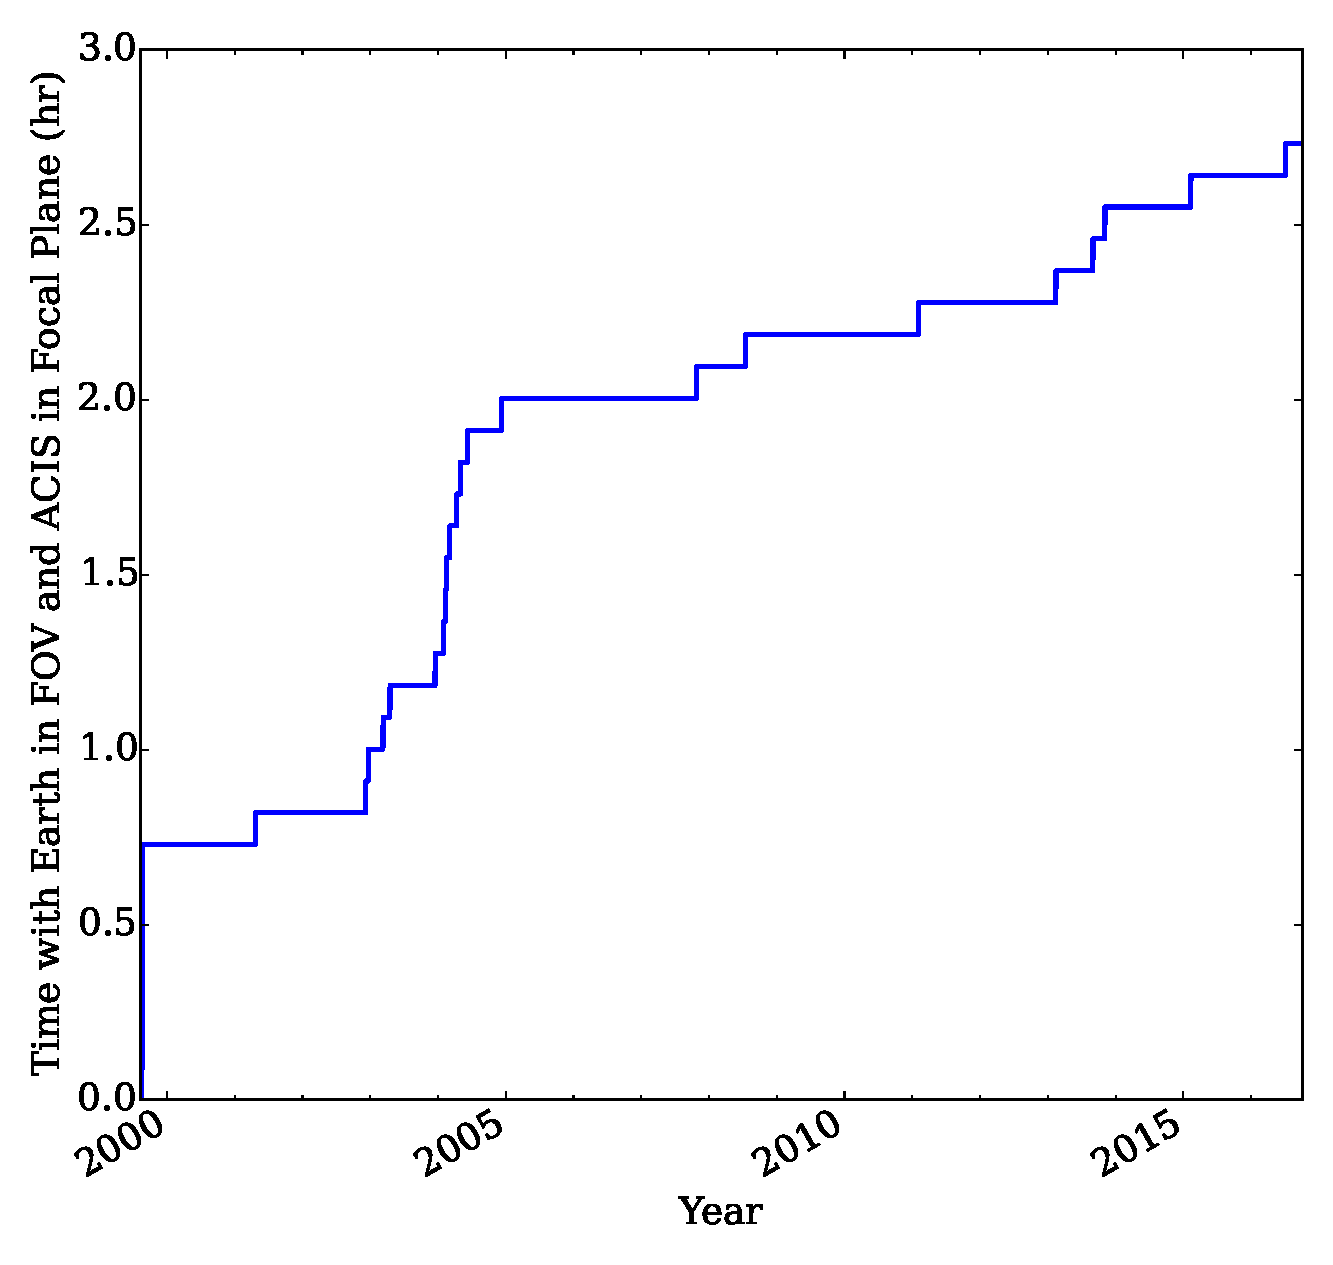
\includegraphics[width=0.7\textwidth]{time_accum.eps}
\caption{Accumulation of time with Earth in the FOV and ACIS in the focal plane over the duration of the mission.\label{fig:time_accum}}
\end{center}
\end{figure}

We assume that the UV photons are reflected from the HRMA onto the focal plane with 100\% efficiency,
so the effective area is $A_{\rm eff} = 1145$~cm$^2$. The ``plate scale'' $\Delta{S}$ of the ACIS focal plane is
0.0205"/$\mu$m. The accumulated fluences of photons which can break H-C and C-C bonds are then, respectively:

\begin{eqnarray}
H_{\rm H-C} &=& I_{\rm H-C}A_{\rm eff}(\Delta{S})^2\Delta{T} = 4.06 \times 10^{12}~{\rm photons~cm^{-2}} \\
H_{\rm C-C} &=& I_{\rm C-C}A_{\rm eff}(\Delta{S})^2\Delta{T} = 3.38 \times 10^{15}~{\rm photons~cm^{-2}}\label{eqn:fluence}
\end{eqnarray}

\noindent
where the number of photons which can break C-C bonds is much higher due to the steep increase in intensity of these photons at wavelengths longer than $\sim$3000~${\rm \AA}$ (Figure \ref{fig:bright_earth_intensity}). Since any photon than can break a C-C bond can also break a H-C bond, we may estimate the total fluence of bond-breaking photons as simply $H = H_{\rm C-C}$.

We can now make a rough estimate of the amount of contaminant that could be polymerized by these photons. It
will be convenient to express this in terms of the surface mass density of C, since this is directly
measureable from calibration studies. Assuming 100\% efficiency (e.g., that each UV photon which impinges upon the OBFs breaks a bond), and that the number of photons required to polymerize $N$ molecules is simply $N-1 \approx N$ (for large $N$), the surface mass density of $C$ that is in the form of polymerized material is then given by:

\begin{equation}\label{eqn:pred_poly}
\sigma_{\rm C} = HN_{\rm C}m_{\rm C}/N_A = 0.067N_{\rm C}~\upmu{\rm g~cm}^{-2}
\end{equation}

\noindent
for $N_{\rm C} = 17$, $\sigma_{\rm C} = 1.14$~$\upmu$g~cm$^{-2}$, which is a small fraction of the mass density
of the contaminant present on the OBFs (Figure \ref{fig:contam_buildup}).

\subsection{UV Flux from Stars}

The next source of UV flux we will consider is that from bright stars. We first examined O stars which have tabulated fluxes in the International Ultraviolet Explorer (IUE) data archive\footnote{\url{https://archive.stsci.edu/iue/}} with apparent magnitudes of 6 or less which have also been observed by \chandra. We also chose to examine the UV flux from other stars which were observed by \chandra~by filtering on the ``Stars and WD'' Science Category of the \chandra~Data Archive, and which also have tabulated spectra in the IUE archive. In both cases, we only examined sources which fell witin 1' of the aimpoint for that observation. The list of stars that were examined, their UV fluxes, and the \chandra~exposure times are given in Table \ref{tab:star_fluxes}. The most significant UV fluences in this sample are from the stars of the Trapezium, which has been observed by \chandra~for $\sim$1~Ms.

\begin{table*}
\caption{Fluxes and Exposure Times for Bright UV Stars\label{tab:star_fluxes}}
\begin{center}
\begin{tabular}{lll}
\hline
\hline
Star & Flux (1150-3445~${\rm \AA}$, photons~s$^{-1}$~cm$^{-2}$) & Exposure Time (ks) \\
\hline
HD37468 & 393502.62 & 12.96 \\
HD36861 & 392165.58 & 9.46 \\
HD57061 & 155969.13 & 97.88 \\
HD38666 & 146539.38 & 115.81 \\
HD37022$^*$ & 101673.45 & 1040.00 \\
HD37020$^*$ & 19373.59 & 1040.00 \\
HD37023$^*$ & 17551.96 & 1040.00 \\
HD135379 & 14217.68 & 19.05 \\
HD152248 & 10694.30 & 120.57 \\
HD91969 & 10554.96 & 70.87 \\
HD37021$^*$ & 5365.84 & 1040.00 \\
HD24534 & 5230.20 & 111.09 \\
HD46150 & 5008.62 & 75.00 \\
HD124314 & 4578.83 & 27.90 \\
HD193793 & 906.34 & 79.60 \\
\hline
\multicolumn{3}{p{.6\textwidth}}{$^*$ Trapezium star cluster}
\end{tabular}
\end{center}
\end{table*}


In keeping with our ``worst case'' approach, we assume that each source is observed at the aimpoint and that the UV flux is spread out over an area on the OBFs corresponding to the outline of the standard \chandra~dither pattern of 32$\times$32 pixels, or 15.74 square arcseconds. For each source, we use the flux of UV shortward of 3445~${\rm \AA}$ (the energy required to break C-C bonds), down to $\sim$1150~${\rm \AA}$, the lower-wavelength limit of IUE.

Summing the contributions from all of our sources together, and using Equation \ref{eqn:fluence} we find a total fluence of $H = 9.14 \times 10^{15}$~photons~cm$^{-2}$. As for the previous calcuation, we can determine the surface mass density of C corresponding to the amount of polymerized contaminant, assuming 100\% efficiency. Using Equation \ref{eqn:pred_poly}, we find $\sigma_{\rm C} = 3.10$~$\upmu$g~cm$^{-2}$, slightly higher than the predicted amount resulting from the bright Earth, but still far smaller than the actual surface mass density of the contaminant.

\subsection{UV Flux from Solar System Objects}

\section{Summary}

We have presented a series of calculations of the estimated UV fluence which has impinged on the ACIS OBFs
over the lifetime of the mission. We have determined that there has not been a sufficient amount of UV fluence
to polymerize a significant amount of the contaminant. The following limitations of our study must be bore in mind:

\begin{itemize}
\item Throughout this memo, we assumed that sufficiently energetic UV photons polymerize contaminant with 100\% efficiency, which is not likely to be the case.
\item We have not considered other sources of UV flux, such as the cosmic UV background or that of diffuse sources which have been observed by \chandra.
\item We have assumed that the HRMA is 100\% reflective to UV photons.
\end{itemize}

We are confident that relaxing some of these assumptions and adopting more detailed calculations will not change our conclusions, since most of these assumptions result in an {\it overestimate} of the polymerization of the contaminant.

\end{document}
